\documentclass[a4j]{jarticle}%[a4j]
%-------Package--------------
%you can add package
\usepackage{wrapfig}
\usepackage{amsmath,amssymb,bm,latexsym,amsfonts,mathrsfs}%equation
\usepackage[dvipdfmx]{graphicx}%pdf
\usepackage[dvipdfmx]{color}
\usepackage{multicol}
\usepackage{here}
%\renewcommand{\figurename}{Fig}%fig name
%\renewcommand{\refname}{[Reference]}%Reference name
%-------margin-------------
% you must not change "margin"
\usepackage[top=20truemm,bottom=20truemm,left=20truemm,right=20truemm]{geometry}%margin 20mm all side


%-------for thesis ------------
%you may not change "for thesis"
\makeatletter
\def\section{\@startsection {section}{1}{\z@}{-2.0ex plus -1ex minus
-.2ex}{0.3ex plus .2ex}{\normalsize\bf}}%section bf and section margin if you need more margin after section number you change ex parameter
 \def\@maketitle{%
 \begin{center}%
 \let\footnote\thanks
   {\large \@title \par}%title font large=12pt
 \end{center}%title
   \mbox{}\hfill%
   {
     \begin{tabular}[t]{r}%right side
       \@author
     \end{tabular}\par}%author
 \vskip\Cvs%
 }


\makeatother
%-------Thesis Title and Author Name------------
\title{{{ \gt{非対称}\sf SNR~G350.1-0.3}{\gt におけるイジェクタ噴出速度の測定}}\\ {\sf Measurement of ejecta velocity in an irregular galactic supernova remnant G350.1-0.3}}
\author{{\gt 湯澤~洋治}\\ \noindent{\gt 指導教員~~内山~泰伸}}%\gt only for Japanese
\date{}



%%%%%%%%%%%%%%%%%%%%%%%%%%%%%%%%%%%%%
%%%%%%  New Command		%%%%%%%%%%%%%%%%
\newcommand{\headfont}{\gtfamily\sffamily\bfseries}
\renewcommand{\figurename}{Fig.}

%\def\pbk{\hbox{particle background}}


\parindent = 10pt
%%%%%%%%%%%%%%%%%%%%%%%%%%%%
%-------Body------------
\begin{document}
\maketitle\thispagestyle{empty}
\pagestyle{empty}



%%%%%%%%%%%%%%%%%%%%%%%%%%%%
%-------はじめに------------
\section{{\sf {\gt はじめに}}}

 太陽の8倍以上の質量を持つ星は、内部での核融合反応による熱エネルギーにより自身の重力を支えている。
反応が進み、中心部で鉄が生成されると、鉄は安定であるためそれ以上核融合が進まなくなるため、急激に内部圧力が下がる。
これにより、外層を支えきれなくなり、重力崩壊を起こす。さらに内部が高密度となると、中心部に中性子の核が残り、落ちこんでくる外層が中心核表面で跳ね返されることで外側に向かう強い衝撃波が形成される。
この衝撃波が、ついには外層を吹き飛ばし、超新星爆発を起こす。近年のシミュレーションでは、爆発前の星の形状の非対称性や星内部の乱流状態による爆発の非球対称性が噴出物の分布に反映されると考えられている。本研究では、X線で観測される形状が非球対称な超新星残骸G350.1-0.3において、超新星爆発によって生じた噴出物の速度を輝線のドップラーシフトから求めることで非球対称な超新星爆発メカニズムに迫る事を目的としている。


%%%%%%%%%%%%%%%%%%%%%%%%%%%%
%------- Aboout SNR  ------------
\section{{\sf {\gt 超新星残骸~\sf{G350.1-0.3}}}}
 G350.1-0.3は(RA,Dec)=(17h21m05s,-37$^\circ$.27)に位置する年齢1000--2000歳の若い超新星残骸である。これまで赤外、電波及びX線で観測されており、それぞれの波長でその特異な形状が異なることが確認されている。日本のX線観測衛星すざくによる観測\cite{Yasumi2014}では、鉄より大きな質量の$\rm{Ni}$が検出されており、非対称な爆発がスペクトル解析から示唆されている。
また、本天体はFig\ref{fig:spec_reg}左図のように極端に非対称な形状をとっていることから、超新星爆発における非対称性を噴出物の分布を引き起こすメカニズムに迫るための重要な天体の1つだと考えられる。


 

%%%%%%%%%%%%%%%%%%%%%%%%%%%%
%-------  Chandra  ------------
\section{{\sf {Chandra~X\gt {線観測衛星}}}}
 Chandra~X線観測衛星は1999年にNASAが打ち上げた衛星である。Chandraには10枚のCCDで構成されるACIS(Advanced CCD Imaging Spectrometer)、マイクロチャンネルプレートからなるHRC(High Resolution Camera)、高エネルギー透過型回折格子HETG(High Energy Transition Grating)と低エネルギー透過型回折格子LETG(Low Energy Transition Grating)という4つの観測機器が搭載されている。
ACISには2$\times$2のCCDからなるACIS-Iと1$\times$6のCCDからなるACIS-Sがある。ACISの特徴は空間分解能が視野中心で約0.5秒角であることと、観測できるエネルギー範囲が$\sim 10$keVまでであることである。
今回、解析に用いたのはこれらのうち撮像と分光が可能なACISを用いて観測されたデータのみである。


%%%%%%%%%%%%%%%%%%%%%%%%%%%%
%------- Chandra analysis ------------
\section{{\sf{Chandra} {\gt による\sf{X} \gt 線解析}}}
 今回、Chandraでによって、2009年5月21日にACIS-Sを用いて82.97~ks観測されたデータとNASAが提供するCIAO(version~4.9)、Xspec(version~12.9)を使用し、解析を行った。

%%%-----------------------------%%%%%
はじめに、超新星残骸をFig\ref{fig:spec_reg}のように放射が明るい3つの領域(東側・北側・南側)に分割し、スペクトル解析を行った。スペクトルモデルは星間吸収モデルとしてwabs、連続成分として制動放射、輝線には複数のガウシアンを考慮した$\rm{wabs \times(bremss+gaussian)}$と赤方偏移$z\sim v/c$を考慮したガウシアンをSi、S、Arに適用した$\rm{wabs \times(bremss+zgaussian)}$である。
解析結果より、Si、S、Arのそれぞれの領域での視線方向の速度を求めた。\\
それぞれの輝線のエネルギー中心値を$E$とすると、ドップラーシフトがない場合に期待されるエネルギーを$E_{0}=E_{East}$として、視線方向の速度は
\begin{align}
  \frac{v}{c} = \frac{| E - E_0 |}{E_0} \label{doppler-equation}
\end{align}
として求められる。解析の結果をFig\ref{fig:velo}に示す。\\

%%%------region figure-----------%%%%%
\begin{figure}[h]
\begin{center}
\begin{tabular}{cc}

\begin{minipage}{0.5\hsize}
\begin{center}
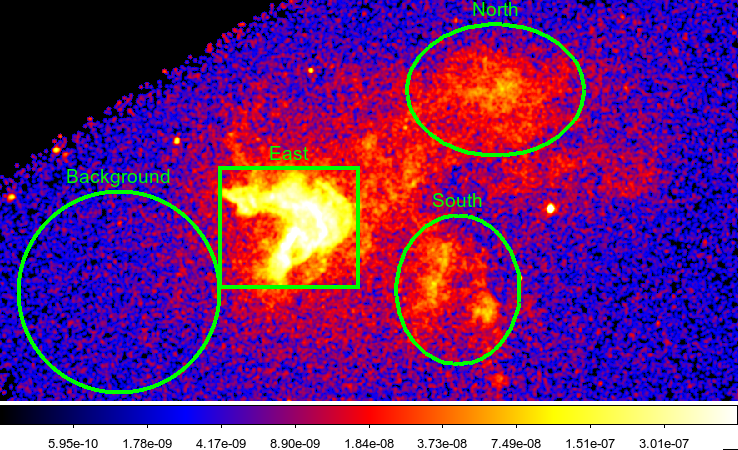
\includegraphics[scale=0.35]{./spectral_region.png}
\end{center}
\end{minipage}

\begin{minipage}{0.5\hsize}
\begin{center}
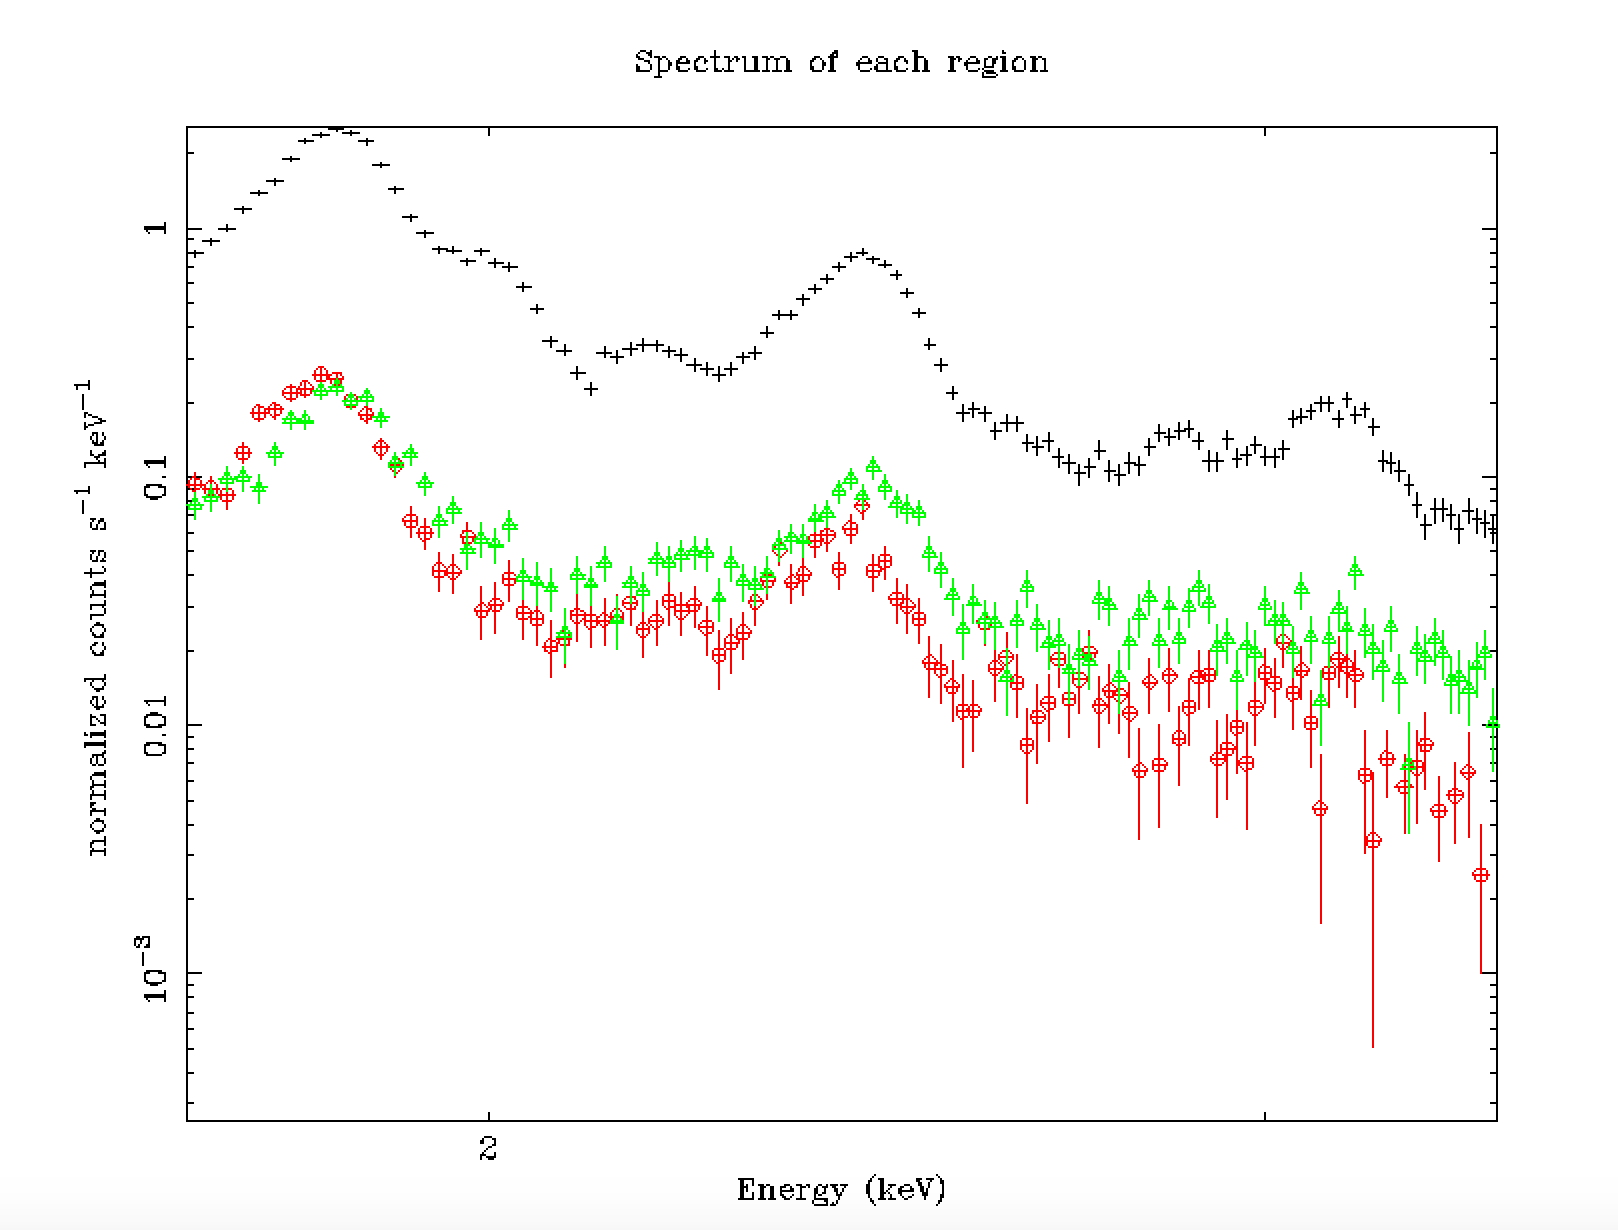
\includegraphics[scale=0.3]{./spectrum_xspec.png}
\end{center}
\end{minipage}
\end{tabular}
\caption{左図:\sf{Chandra}によるG350.1-0.3のフラックスイメージ$\rm{(0.5-8.0~keV)}$、右図:\sf{Chandra}による\sf{SNR}の各領域のスペクトル$\rm{(1.7-3.4~keV)}$ 黒線(マーカー:$+$):東側のスペクトル、赤線($\bigcirc$):南側のスペクトル、緑線($\bigtriangleup$):北側のスペクトル}
\label{fig:spec_reg}
\end{center}
\end{figure}


\begin{wrapfigure}[20]{r}[-20mm]{70mm}
\begin{center}
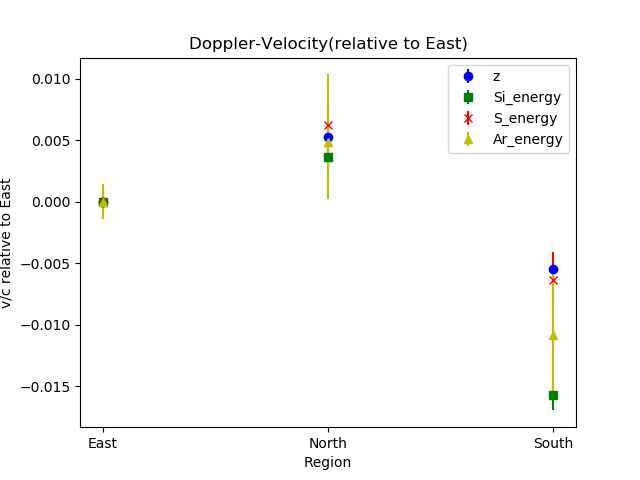
\includegraphics[scale=0.6]{./vel_lineofsight.png}
\caption{ドップラー効果から求めた東側の放射領域に対する各元素の速度}
\label{fig:velo}
\end{center}
\end{wrapfigure}

\newpage
%------- Chandra analysis ------------
\section{{\sf {\gt 議論}}}
 今回のChandraの観測データの解析によって、超新星残骸G350.1-0.3において、南側と北側の領域がそれぞれ視線方向に対して、遠ざかる向きと近づく向きに運動していることがわかった。
この結果から、赤方偏移$\it{z}$を用いて視線方向の速度を求めると、南と北はそれぞれ、$v_{\rm{South}} \sim 1640^{+150}_{-130}$~km/s、$v_{\rm{North}} \sim 1570^{+330}_{-240}$~km/sであるとわかる。さらに、天体までの距離$\it{d}$を$d \sim 4.5~\rm{kpc}$\cite{Gaensler2008}と仮定すると、天体までの距離と楕円の長軸の大きさを用いて、南と北の領域の大きさはそれぞれ、$R_{South} \sim 0.95$~pc、$R_{North} \sim 1.14$~pcとなる。
このことから、巨大なプラズマ塊が光速の$\sim \pm 0.5 \%$程度で運動していることがわかる。この結果から、この超新星残骸が極端に非対称な超新星爆発によって誕生したことが強く示唆される。\\
 今後はESAのXMM-Newtonを用いた同様の解析によって、今回のChandraのデータを用いた解析による結果を確認することを予定している。この他、ドップラー効果の面から非対称性爆発が示唆されたことから、Chandraの空間分解能を活かし、より細かな領域に分割し、それぞれの領域でスペクトル解析することで、どのような超新星爆発モデルによってこの超新星爆発が再現できるのか既存の理論と照らし合わせて確かめていきたい。


%%%%%%%%%%%%%%%%%%%%%%%%%%%%
%-------  Reference  -----------

\vspace{-1mm}
\setlength{\columnsep}{0.4pt}
%\setlength{\columnseprule}{0.4pt}
\setlength{\columnwidth}{10mm}
\begin{thebibliography}{5}
  \vspace{-5mm}
  \begin{multicols}{2}
    \vspace{-2mm}
		\bibitem{toshikisato}
		Toshiki Sato 博士論文 2018
    \label{toshikisato}

    \vspace{-2mm}
    \bibitem{Yasumi2014}
    Yasumi, M. et al. 2014, Pasj, 66, 68
    \label{Yasumi2014}

    \vspace{-2mm}
    \bibitem{2010ApJ...725..894H}
    Hayato, A. et al. 2010, Apj, 725, 894
    \label{2010ApJ...725..894H}

    \vspace{-2mm}
    \bibitem{Gaensler2008}
    Gaensler, B.~M. et al. 2008, ApjL, 680, L37
    \label{Gaensler2008}


  \end{multicols}

\end{thebibliography}



\end{document}
